\section{Ziel}
In diesem Versuch soll eine Kuper-Röntgenröhre auf ihr Emissionsspektrum untersucht und die Bragg-Bedingung überprüft werden.
Außerdem sollen diverse Absorptionsspektren gemessen und ihre Abschirmkonstanten bestimmmt werden.


\section[Theorie]{Theorie\footnote[1]{Unter Verwendung von \cite[]{man:v602}.}}

\subsection{Erzeugung von Röntgenstrahlung}
Röntgenstrahlung wird erzeugt, indem in einer evakuierten Röhre Elektronen durch den glühelektrischen Effekt aus einer Kathode gelöst werden.
Diese Elektronen werden durch eine angelegte Spannung zu einer Anode hin beschleunigt.
Beim Auftreffen auf die Anode entsteht Röntgenstrahlung, wobei das kontinuierliche Bremsspekttrum und die diskrete charakteristische Röntgenstrahlung des Anodenmaterials unterschieden werden.

\noindent
Bei der Bremsstrahlung werden die Elektronen im Coulombfeld des positives Atomkerns abgebremst.
Durch die Abremsung wird ein Photon emittiert, dessen Energie genau der verloren kinetischen Energie des jeweiligen Elektrons entspricht.
Da nicht alle Elektronen die gleiche Energie abgeben, entsteht ein kontinuierliches Energiespektrum, das eine obere Grenze an der Stelle hat,
bei der die gesamte kinetische Energie übertragen wird.
Für die minimale Wellenlänge folgt demnach bei vollständiger Abbremsung des Elektrons
\begin{align}
    \lambda_\text{min} = \frac{h \cdot c}{e_0 U},
    \label{eq:wellenlaenge}
\end{align}
wobei $U$ die angelegt Spannung ist.
Die Intensitätsverteilung des Bresmspektrums ist in Abbildung \ref{fig:bremsspektrum} zu sehen.
\begin{figure}[H]
    \centering
    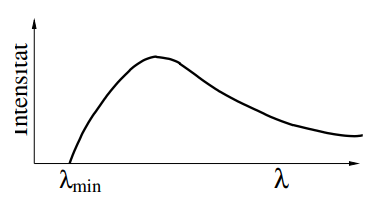
\includegraphics[height = 3.5cm]{Abbildungen/bremsspektrum.png}
    \caption{Intensitätsverteilung in Abhängigkeit der Wellenlänge beim charakteristischen Spektrum \cite[]{man:v602}.}
    \label{fig:bremsspektrum}
\end{figure}

\noindent
Beim charakteristischen Spektrum werden die Anodenatome so ionisiert, dass das beschleunigte Elektron 
ein inneres Schalenelektron heraus löst. 
Wenn das Atom anschließend in seinen Grundzustand zurück wechselt, wird ein Photon mit der Energie 
\begin{align}
    \Delta E = h \cdot \nu = E_\text{m} - E_\text{n}
    \label{eq:energiedifferenz}
\end{align}
emittiert.
Diese Energie entspricht genau der Energiedifferenz zwischen der äußeren Schale m, von der ein Elektron nachrückt, und der inneren Schale n,
aus der ein Elektron zuvor geschlagen wurde. 
Da diese Energien für jedes Material spezifisch nur gewisse diskrete Werte annimmt, ist das resultierende Spektrum diskret.
Dabei werden die einzelnen Linien mit $K_\alpha$, $K_\beta$, $L_\alpha$ bezeichnet.
Die Schale, auf der die Sprünge enden, geben dabei die Buchstaben $K$, $L$, usw. vor während die griechischen Buchstaben angeben, von welcher Schale das 
äußere Elektron stammt.
In Atomen mit mehreren Elektronen erzeugen die Hüllenelektronen und die Wechselwirkungen der Elektronen untereinander eine gewisse Abschirmung von der Kernladung,
sodass das äußere Elektron eine geringere Coulombanziehung erfährt.
Für die Energie eines solchen Elektrons auf der n-ten Schale gilt dann
\begin{align}
    E_\text{n} = - R_\infty z_\text{eff}^2 \cdot \frac{1}{n^2}
    \label{eq:effektive_energie}
\end{align}
mit der effektiven Kernladung $z_\text{eff} = z - \sigma$, der elektronenspezifischen Abschirmkonstanten $\sigma$ und der Rydbergenergie $R_\infty = \qty[]{13.6}{\electronvolt}$.
Für die Energie $E_{K_\alpha}$ ergibt sich dann beispielsweise
\begin{align}
    E_{K_\alpha} = E_2 - E_1 = R_\infty \cdot \left(\left(z-\sigma_1\right) \cdot \frac{1}{1^2} - \left(z-\sigma_2\right) \cdot \frac{1}{2^2}\right).
    \label{eq:k_alpha}
\end{align}

\noindent
Durch den Bahndrehimpuls und den Spin haben die äußeren Elektronen nicht exakt die gleiche Bindungsenergie, sodass die jeweilige charakteristische Linie in eine
Feinstruktur aufgelöst wird, die jedoch mit dem hier verwendeten Versuchsaufbau nicht detektiert werden kann.
Messbar sich hier die $K_\alpha$- und $K_\beta$-Linien der Kuperanode sowie die Bremsstrahlung.





\subsection{Absorption von Röntgenstrahlung}
Bei einer Strahlung mit Energien unterhalb von \qty[]{1}{\mega\electronvolt} sind der Compton- und Photoeffekt die relevanten Prozesse.
In Abbildung \ref{fig:absorption} ist erkennbar, dass der Absorptionskoeffizient für steigende Energien sinkt, aber sprunghaft ansteigt, wenn die Energie der 
Photonen gerade größer als die Bindungsenergie eines Elektrons der nächsten inneren Schale ist.
Die Energien der Schale, aus der das Elektron stammt, wird dabei als Absorptionskante bezeichnet.
Die Lage der Absorptionskanten  $h \nu_\text{abs} = E_\infty - E_\text{n}$ ist dabei nahezu identisch wie die Bindungsenergie.
Aufgrund der Feinstruktur gibt es insgesamt drei L- und eine K-Kante.
Die Bindungsenergie eines Elektrons kann gemäß der Sommerfeldschen Freinstrukturformel 
\begin{align}
    E_\text{n,j} = -R_\infty \left(z_\text{eff,1}^2 \cdot \frac{1}{n^2} + \alpha^2 z_\text{eff,2}^4 \cdot \frac{1}{n^3} \left(\frac{1}{j + \frac{1}{2}} - \frac{3}{4n}\right)\right)
    \label{eq:sommerfeld}
\end{align} 
mit der Sommerfeldschen Feinstrukturkonstante $\alpha$ und dem Gesamtdrehimpuls $j$ des jeweiligen Elektrons.
Für ein Elektron aus der K-Schale ergibt sich die Abschirmkonstante
\begin{align}
    \sigma_K = z - \sqrt{\frac{E_K}{R_\infty} - \frac{\alpha^2 z^4}{4}}.
    \label{eq:abschirmung_k}
\end{align}
Für ein Elektron der L-Schale ist die Herleitung von $\sigma_L$ deutlich komplizierter, da die Abschirmzahl jedes beteiligten Elektrons miteinbezogen werden muss.
Werden zwei Kanten (hier $L_I$ und $L_II$) zusammengefasst, vereinfacht sich die Herleitung etwas und es ergibt sich
\begin{align}
    \sigma_L = z - \sqrt{\left(\frac{4}{\alpha}\sqrt{\frac{\Delta E_L}{R_\infty}} - \frac{5 \Delta E_L}{R_\infty}\right)
    \cdot \left(1 + \frac{19}{32} \alpha^2 \frac{\Delta E_L}{R_\infty}\right)}
    \label{eq:abschirmung_l}
\end{align}
mit der Energiedifferenz $\Delta E_L = E_{L_{II}} - E_{L_{III}}$.


\begin{figure}[H]
    \centering
    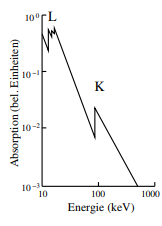
\includegraphics[height= 5.5cm]{Abbildungen/absorption.png}
    \caption[]{Energieabhängigkeit des Absorptionskoeffizienten \cite[]{man:v602}.}
    \label{fig:absorption}
\end{figure}




\subsection{Bragg-Bedingung}
Die Energie $E$ bzw. Wellenlänge $\lambda$ kann durch die Bragg-Reflexion\footnote[2]{Der Begriff \enquote{Reflexion} ist hier sehr irreführend, da es sich tatsächlich um Beugung handelt.}
ermittelt werden.
Wenn Licht auf ein dreidimensionales Gitter (hier LiF-Kristall) trifft,
werden die Photonen an jedem Atom des Gitters gebeugt, wobei die Röntgenstrahlen interferieren.
Unter dem Glanzwinkel $\theta$ tritt dann konstruktive interferenz auf.
Bei einer Gitterkonstante $d$ und der Beugungsordnung $n$ (Kristallschicht, bei der die Beugung stattfindet) gilt dabei die Bragg-Bedingung
\begin{align}
    2 d \sin \theta = n \lambda.
    \label{eq:bragg}
\end{align}
Eine schematische Darstellung der Bragg-Reflexion ist in Abbildung \ref{fig:bragg} zu sehen.

\begin{figure}[H]
    \centering
    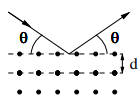
\includegraphics[height = 4cm]{Abbildungen/bragg.png}
    \caption[]{Schematische Darstellung der Bragg-Reflexion \cite[]{man:v602}.}
    \label{fig:bragg}
\end{figure}


\subsection{Vorbereitungsaufgaben}
Der in diesem Versuch verwendete Lif-Kristall hat eine Gitterkonstante von $d = \qty[]{201.4}{\pico\meter}$.

\subsubsection[]{K-Linien und Beugungswinkel bei Kupfer}
%  Energie alpha =  8.04 keV
%  Energie beta =  8.94 keV
%  lambda_k_alpha =  154.20920203134364 pm
%  lambda_k_beta =  138.6847857194634 pm
%  theta_alpha:  22.509902591224215 deg
%  theta_beta:  20.139184010738617 deg
%
%
%# teta_Zn 18.58067369078699
%# teta_Ge 16.09927954595463
%# teta_Br 13.209491136899516
%# teta_Rb 11.683415807687602
%# teta_Sr 11.021875190709254
%# teta_Zr 9.851683102895548
%# sigma_Zn 3.5517350596183093
%# sigma_Ge 3.676565400559749
%# sigma_Br 3.847735266899239
%# sigma_Rb 3.9440375141854815
%# sigma_Sr 3.999052214360077
%# sigma_Zr 4.101347507826553